%! Author = nadutkinfedor
%! Date = 09.01.2024

% Preamble
\documentclass[11pt]{article}
\usepackage[left=2cm, right=1cm, top=2cm, bottom=2cm, bindingoffset=0cm]{geometry}

% Packages
\usepackage[utf8]{inputenc}
\usepackage[russian]{babel}
\usepackage{amsmath}
\usepackage{hyperref}
\usepackage{graphicx}
\usepackage{misccorr}
\usepackage{listings}
\usepackage{xcolor}
\usepackage{titlesec}
\usepackage{minted}
\usepackage{color}
\usepackage{enumitem}
\usepackage{indentfirst}

%listing settings
\definecolor{dkgreen}{rgb}{0,0.6,0}
\definecolor{gray}{rgb}{0.5,0.5,0.5}
\definecolor{mauve}{rgb}{0.58,0,0.82}

\lstset{language=SQL,
    basicstyle={\small\ttfamily},
    belowskip=3mm,
    breakatwhitespace=true,
    breaklines=true,
    classoffset=0,
    columns=flexible,
    commentstyle=\color{dkgreen},
    framexleftmargin=0.25em,
    keywordstyle=\color{blue},
    numbers=none, %If you want line numbers, set `numbers=left`
    numberstyle=\tiny\color{gray},
    showstringspaces=false,
    stringstyle=\color{mauve},
    tabsize=3,
    xleftmargin =1em,
    backgroundcolor=\color{gray!10}
}

\lstset{ %
    backgroundcolor=\color{white},   % choose the background color
    basicstyle=\footnotesize,        % size of fonts used for the code
    breaklines=true,                 % automatic line breaking only at whitespace
    captionpos=b,                    % sets the caption-position to bottom
    commentstyle=\color{dkgreen},    % comment style
    escapeinside={\%*}{*},          % if you want to add LaTeX within your code
    keywordstyle=\color{blue},       % keyword style
    stringstyle=\color{mauve},     % string literal style
}

% link setting
\hypersetup{
    colorlinks=true,
    linkcolor=blue,    % Синий цвет для внутренних ссылок
    filecolor=magenta, % Можно выбрать другой цвет для файлов
    urlcolor=blue      % Синий цвет для URL
}

% Title
\title{DB internals. Третья лекция}
\author{Надуткин Федор }
\date{December 2023}

\titleformat{\section}[block]{\Huge\bfseries\filcenter}{}{1em}{}
\titleformat{\subsection}[block]{\LARGE\bfseries\filcenter}{}{1em}{}
\titleformat{\subsubsection}[block]{\Large\bfseries\filcenter}{}{1em}{}

% Document
\begin{document}

    \maketitle
    \newpage
    \section*{Планирование порядка join}


    \begin{lstlisting}[language=SQL,
        label={lst:join_problem},
        caption={Пример проблемного Join}]
        SELECT
            lineitem.*
        FROM customer
            JOIN orders ON c_custkey = o_custkey
            JOIN lineitem on o_orderkey = l_orderkey
        WHERE
            c_name = 'Ivanov'
    \end{lstlisting}

    \begin{figure}[h!]
        \begin{minipage}{0.5\textwidth}
            \centering
            \includegraphics*[width=0.7\textwidth]{Pictures/Problem/Bad variant}
            \caption{Плохой вариант построения Join}
        \end{minipage}
        \begin{minipage}{0.5\textwidth}
            \centering
            \includegraphics*[width=0.7\textwidth]{Pictures/Problem/Good variant}
            \caption{Хороший вариант построения Join}
        \end{minipage}
        \label{fig:join_problem_pictures}
    \end{figure}

    Как можно видеть из картинок во втором варианте нам нужно хранить в разы меньше промежуточной информации.
    Получается один порядок Join будет гораздо лучше другого.
    Таким образом наш движок должен правильно уметь расставлять порядок Join.

    Попробуем оценить сколько всего существует возможных порядков Join.
    Всего их $= n!$ ---перебор всех возможных расстановок.

    Однако вариант $((a_1 \cdot a_2) \cdot a_3) \cdot a_4 \dots$ не всегда оптимален,
    и зачастую мы хотим также уметь расставлять скобки, как например $(a_1 \cdot a_2) \cdot (a_3 \cdot a_4)$.

    Количество способов расставить скобки равно числу Каталана $C(n-1) = \frac{(2 \cdot n - 2)!}{n! \cdot (n-1)!}$.

    Таким образом количество возможных вариантов равно $n! \cdot C(n-1)$.
    Так для 8 таблиц у нас есть более 17 миллионов альтернатив и растёт оно всё экспоненциально.
    Понятно, что, перебирать все Join у нас физически нет возможности, значит надо использовать эвристики.

    \subsection{Не рассматривать Cross Join}

    Если между таблицами нет соединений, то их Join будет представлен в виде таблицы размером $table_1 \cdot table_2$,
    и скорее всего у нас есть более выгодные альтернативы.

    Однако эта оптимизация может не всегда срабатывать.
    \newpage

    \begin{lstlisting}[h!,language=SQL]
        SELECT *
            FROM sales
                JOIN customer ON sales.cust_id = customer.id
                JOIN sales_date on sales.date_id = sales_date.id
        WHERE sales_date.date = '2024-02-04'
        AND customer.city = 'Tver'
    \end{lstlisting}

    Согласно оптимизации мы должны сделать следующий порядок $customer \cdot sales \cdot date$,
    однако в таком случае придётся держать в памяти большую таблицу.
    С другой стороны можно в начале соединить \texttt{customer} и \texttt{date}, получив маленькую табличку,
    а затем связать с \texttt{sales}.

    \begin{figure}[h!]
        \centering
        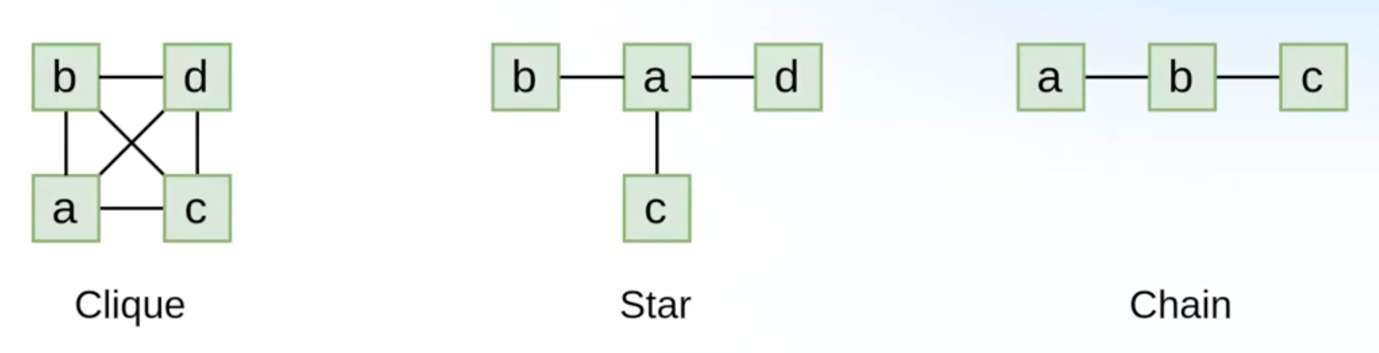
\includegraphics[width=0.7\textwidth]{Pictures/Cross Join/Topology}
        \caption{Возможные топологии соединений}
    \end{figure}

    Данная оптимизация по-разному влияет на разные топологии.
    Например, клике она никак не помогает, а вот для \texttt{Chain} --- количество порядков уменьшается,
    так для 10 таблиц надо будет рассмотреть лишь 2,5 миллиона вариантов.

    \subsection{Динамическое программирование}

    \subsubsection{Снизу вверх}

    \begin{figure}[h!]
        \begin{minipage}{0.2\textwidth}
            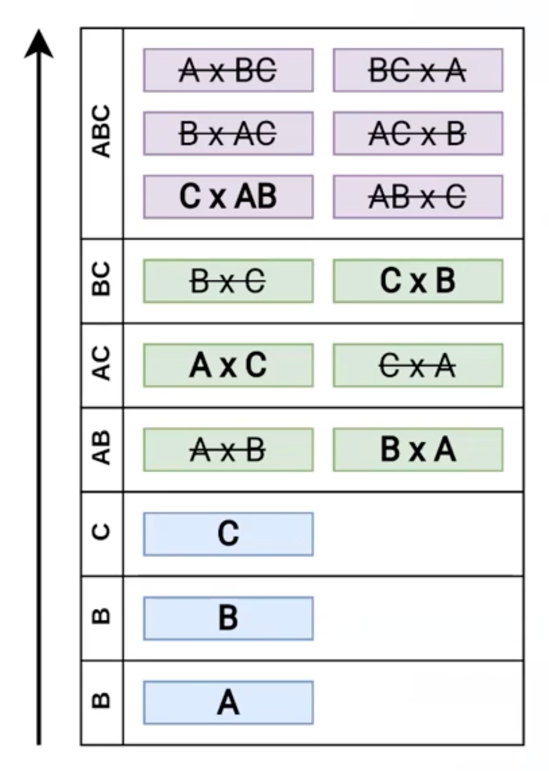
\includegraphics[width=\textwidth]{Pictures/Dynamic Programming/Bottom up/Bottom up}
            \caption{Bottom up подход}
        \end{minipage}
        \begin{minipage}{0.8\textwidth}
            \centering
            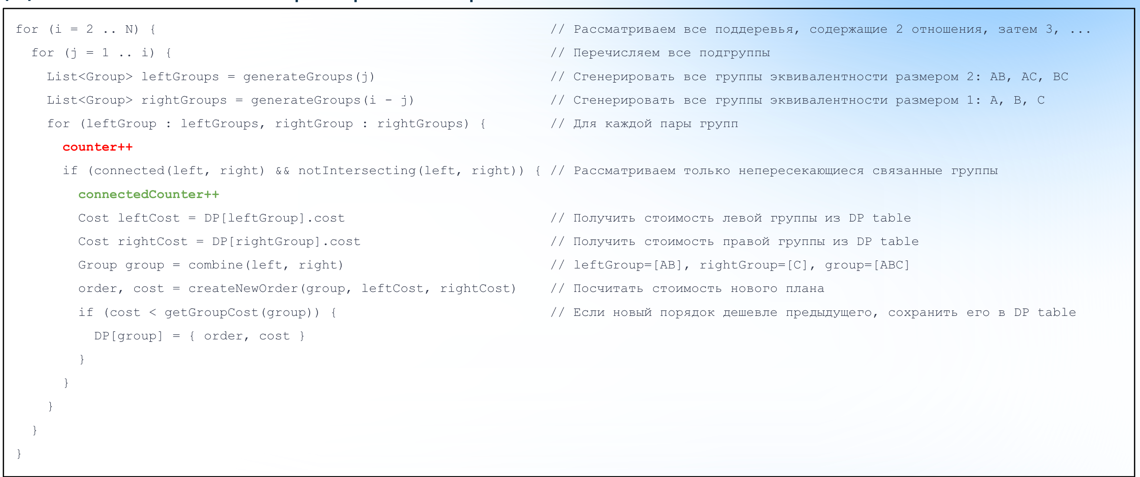
\includegraphics[width=\textwidth]{Pictures/Dynamic Programming/Bottom up/DBSize}
            \caption{DPSize}
        \end{minipage}
    \end{figure}

    \begin{itemize}
        \item Cтроим оптимальные группы для каждой из выборок размера $\leq k$.
        \item Переходим к $k+1$ группам, перебирая левую группу (размера $\leq k$) и автоматически подобранным к ней правым группам.
        \item Хорошо работает для разрешенных графов.
        \item Порядок обхода \textbf{A, B, C, AB, AC, BC, ABC}
    \end{itemize}

    Другим вариантом \texttt{Bottom up} подхода является \textbf{DPSub} --- перебор масок.

    \begin{figure}[h!]
        \centering
        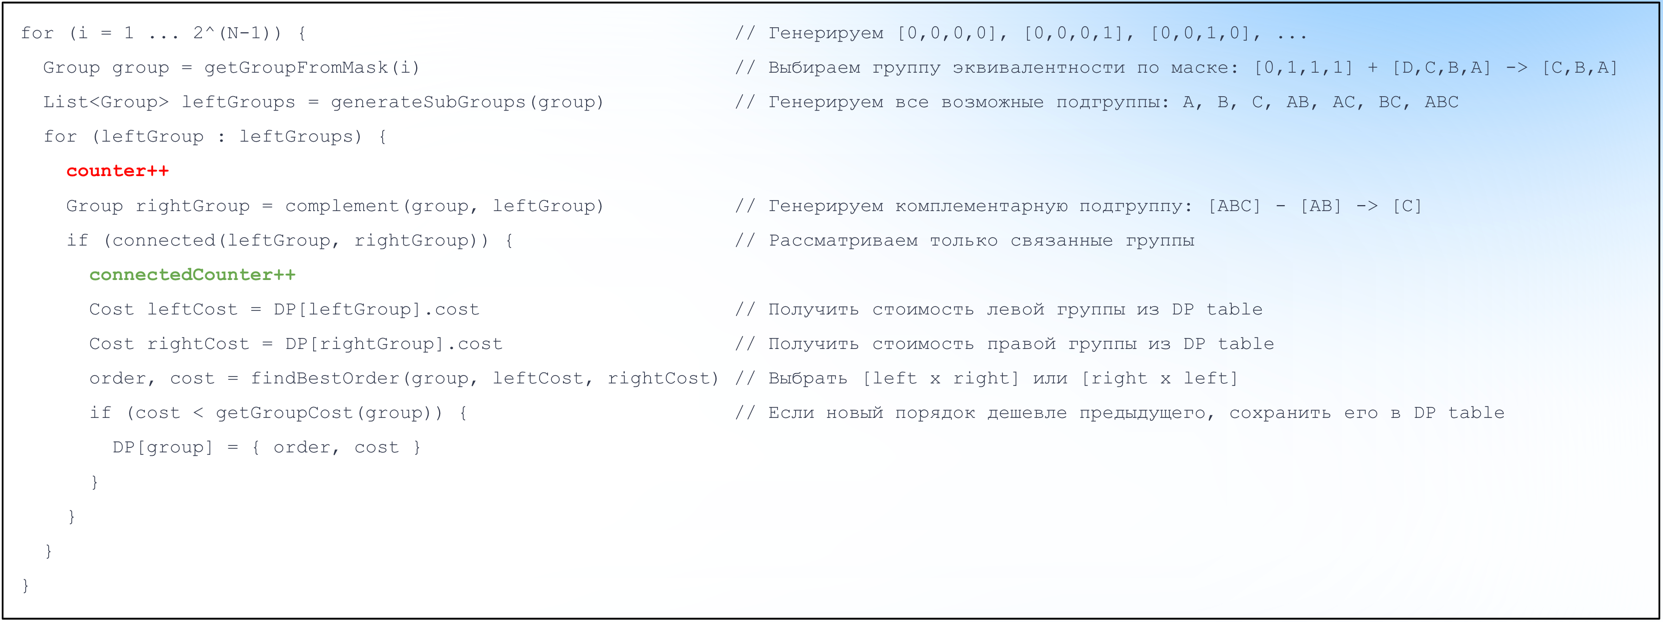
\includegraphics[width=\textwidth]{Pictures/Dynamic Programming/Bottom up/DPSub}
        \caption{DPSub}
    \end{figure}

    \begin{itemize}
        \item Хорошо работает для графов с большим количеством рёбер.
        \item Порядок обхода \textbf{A, B, AB, C, AC, AB, ABC}.
    \end{itemize}

    \textbf{Проблемы подхода:}
    \begin{itemize}
        \item Всё также NP полный.
        \item Каждый раз когда красный счётчик увеличивается, а зелёный нет --- мы делаем бесполезную работу.
        \item Не позволяет эффективно учитывать свойства, которые приходят сверху.
        Например, мы можем не сохранить сортировку для будущего Join, который был бы нам ясен выше и не получится сделать MergeJoin.
    \end{itemize}

    \subsubsection{Сверху вниз}

    \begin{figure}[h!]
        \centering
        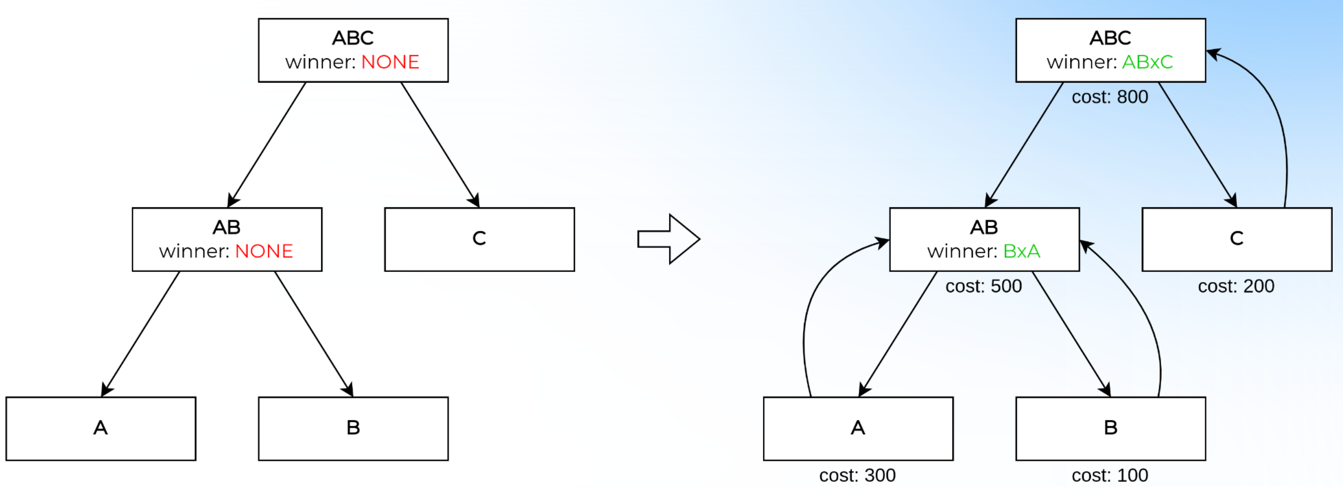
\includegraphics[width=0.5\textwidth]{Pictures/Dynamic Programming/Top down/Граф обхода}
        \caption{Граф для top-down алгоритма.}
    \end{figure}

    В данном подходе мы используем MEMO.

    \textbf{Оптимизации:}

    \begin{itemize}
        \item \textbf{Upper-bound pruning} - не добавлять оператор в MEMO, если ясно, что его стоймость уже выше оставшегося бюджета.
        Например, если мы знаем, что на данный момент оптимальный план стоит 800, просканировать только A, стоит 300, то мы не будем рассматривать планы, дороже 500.
        \item \textbf{Lower-bound pruning} - не исследовать группу дальше, если ясно, что её стоймость уже не улучшить.
        (Однако такое на практике такое почти нигде не сделано, так как не ясно до конца как оценить).
        \item Запускать параллельно, после того, как разделили на группы.
    \end{itemize}

    \textbf{Проблемы:}

    \begin{itemize}
        \item Сложнее для реализации.
        \item Потребляют больше памяти (из-за MEMO).
    \end{itemize}
    
    \begin{figure}[h!]
        \centering
        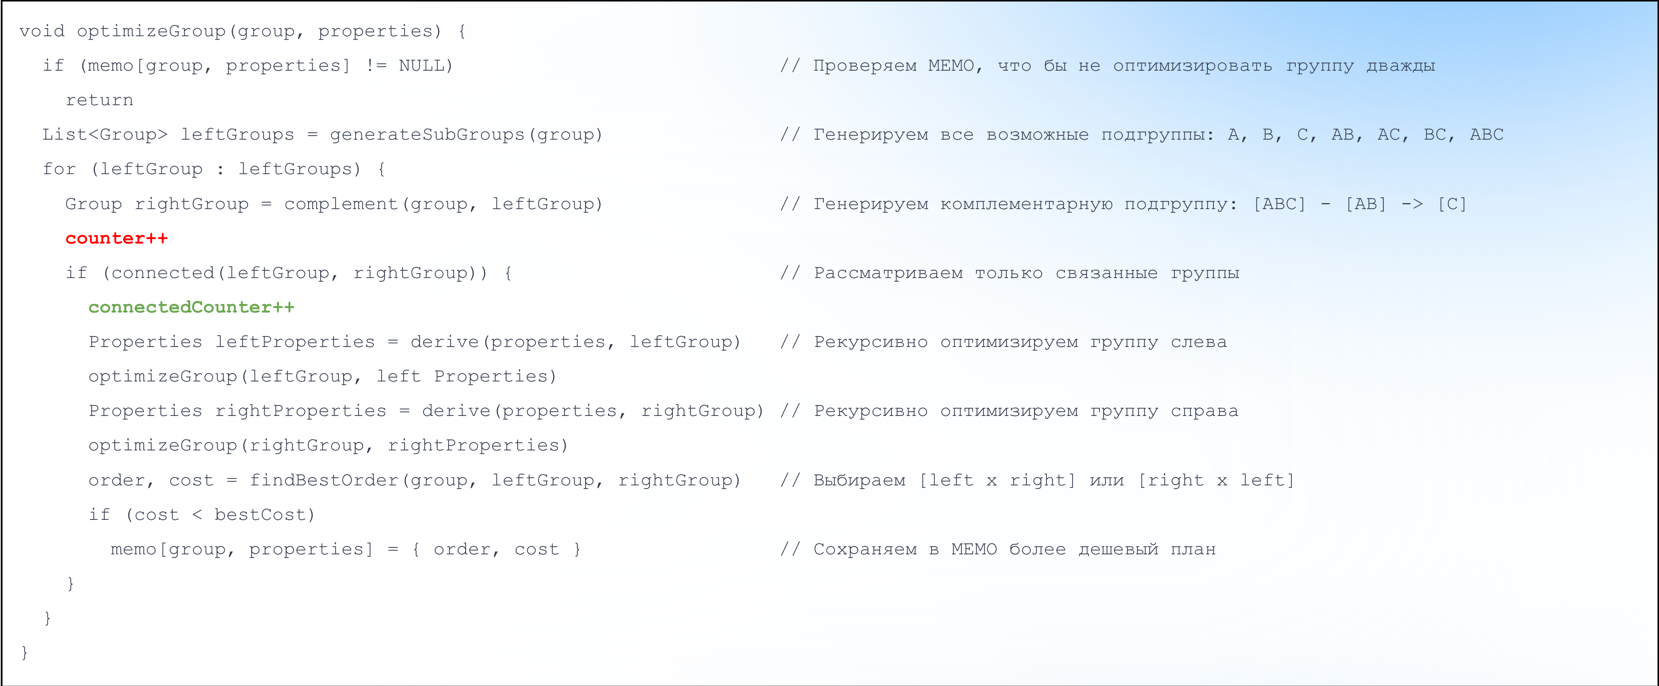
\includegraphics[width=\textwidth]{Pictures/Dynamic Programming/Top down/Код top down}
        \caption{Наивная реализация top down алгоритма}
    \end{figure}

    \href{https://www.semanticscholar.org/paper/Effective-and-Robust-Pruning-for-Top-Down-Join-Fender-Moerkotte/1953bb7c5f5f74b36588dfd0a6fbdb7098cdc0c6}{Современная реализация алгоритма}

    \subsection{Планирование join с помощью правил}

    \begin{figure}[h!]
        \centering
        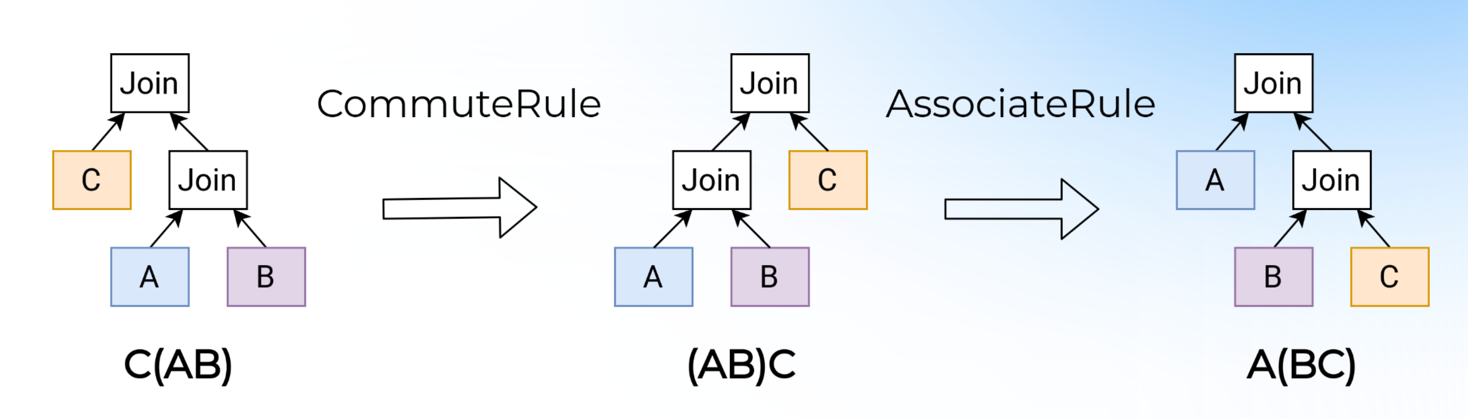
\includegraphics[width=0.6\textwidth]{Pictures/Rules/Деревья}
        \caption{Примеры правил}
    \end{figure}

    \begin{itemize}
        \item \texttt{CommuteRule}: AB $\rightarrow$ BA
        \item \texttt{AssociateRule}: (AB)C $\rightarrow$ A(BC)
        \item \texttt{RotateRule}: (AB)C $\rightarrow$ (AC)B
    \end{itemize}

    \texttt{CommuteRule} и \texttt{AssociateRule} достаточно для генерирования остальных правил.

    Однако применяя правило мы постоянно будем приходить в состояния в которых уже бывали.
    Причём обычно бороться с этим гораздо хуже, чем работать с предыдущими вариантами.
    
    \begin{figure}[h!]
        \centering
        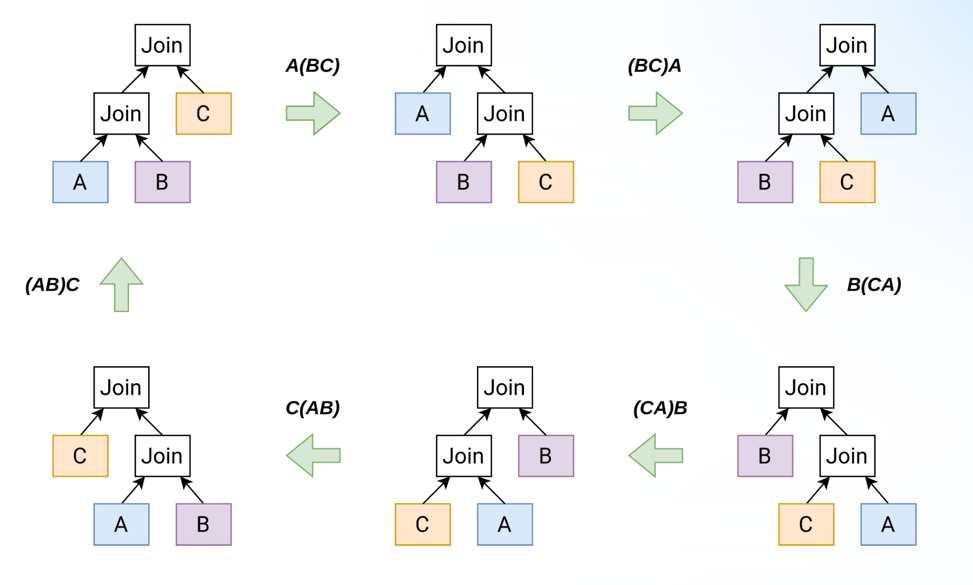
\includegraphics[width=0.6\textwidth]{Pictures/Rules/Циклы}
        \caption{Пример прихода в цикл используя правила.}
    \end{figure}
    
    \textbf{Как бы хотелось}
    \begin{itemize}
        \item Генерировать все возможные планы.
        \item Top-Down обход оптимально использует свойства.
        \item Top-Down эффективно реализует branch-and-bound pruning.
    \end{itemize}
    
    \textbf{Как на самом деле}
    \begin{itemize}
        \item Генерируем все планы для маленьких запросов.
        \item Рассмотрение всех свойств происходит эвристически, не всегда мы используем свойства оптимально.
        \item Branch-and-bound pruning мало где реализован.
        \item Legacy мешает.
    \end{itemize}
\end{document}